%% abtex2-modelo-trabalho-academico.tex, v-1.9.2 laurocesar
%% Copyright 2012-2014 by abnTeX2 group at http://abntex2.googlecode.com/ 
%%
%% This work may be distributed and/or modified under the
%% conditions of the LaTeX Project Public License, either version 1.3
%% of this license or (at your option) any later version.
%% The latest version of this license is in
%%   http://www.latex-project.org/lppl.txt
%% and version 1.3 or later is part of all distributions of LaTeX
%% version 2005/12/01 or later.
%%
%% This work has the LPPL maintenance status `maintained'.
%% 
%% The Current Maintainer of this work is the abnTeX2 team, led
%% by Lauro César Araujo. Further information are available on 
%% http://abntex2.googlecode.com/
%%
%% This work consists of the files abntex2-modelo-trabalho-academico.tex,
%% abntex2-modelo-include-comandos and abntex2-modelo-references.bib
%%

% ------------------------------------------------------------------------

\documentclass[
	% -- opções da classe memoir --
	12pt,				% tamanho da fonte
	% openright,			% capítulos começam em pág ímpar (insere página vazia caso preciso)
	oneside,			% para impressão apenas no anverso (apenas frente). Oposto a twoside
	a4paper,			% tamanho do papel. 
	% -- opções da classe abntex2 --
	%chapter=TITLE,		% títulos de capítulos convertidos em letras maiúsculas
	%section=TITLE,		% títulos de seções convertidos em letras maiúsculas
	%subsection=TITLE,	% títulos de subseções convertidos em letras maiúsculas
	%subsubsection=TITLE,% títulos de subsubseções convertidos em letras maiúsculas
	% -- opções do pacote babel --
	english,			% idioma adicional para hifenização
	%french,				% idioma adicional para hifenização
	%spanish,			% idioma adicional para hifenização
	brazil				% o último idioma é o principal do documento
	]{abntex2ppgsi}

% ---
% Pacotes básicos 
% ---
% \usepackage{lmodern}			% Usa a fonte Latin Modern			
% \usepackage[T1]{fontenc}		% Selecao de codigos de fonte.
\usepackage[utf8]{inputenc}		% Codificacao do documento (conversão automática dos acentos)
\usepackage{indentfirst}		% Indenta o primeiro parágrafo de cada seção.
\usepackage{color}				% Controle das cores
\usepackage{graphicx}			% Inclusão de gráficos
\usepackage{microtype} 			% para melhorias de justificação
\usepackage{pdfpages}     %para incluir pdf
\usepackage{algorithm}			%para ilustrações do tipo algoritmo
\usepackage{mdwlist}			%para itens com espaço padrão da abnt
\usepackage[noend]{algpseudocode}			%para ilustrações do tipo algoritmo
		
% ---
% Pacotes adicionais, usados apenas no âmbito do Modelo Canônico do abnteX2
% ---
\usepackage{lipsum}				% para geração de dummy text
% ---

% ---
% Pacotes de citações
% ---
\usepackage[brazilian,hyperpageref]{backref}	 % Paginas com as citações na bibl
\usepackage[alf]{abntex2cite}	% Citações padrão ABNT

% --- 
% CONFIGURAÇÕES DE PACOTES
% --- 

% ---
% Configurações do pacote backref
% Usado sem a opção hyperpageref de backref
\renewcommand{\backrefpagesname}{Citado na(s) página(s):~}
% Texto padrão antes do número das páginas
\renewcommand{\backref}{}
% Define os textos da citação
\renewcommand*{\backrefalt}[4]{
	\ifcase #1 %
		Nenhuma citação no texto.%
	\or
		Citado na página #2.%
	\else
		Citado #1 vezes nas páginas #2.%
	\fi}%
% ---

% ---
% Informações de dados para CAPA e FOLHA DE ROSTO
% ---

%-------------------------------------------------------------------------
\instituicao{
	UNIVERSIDADE DE SÃO PAULO
	\par
	ESCOLA DE ARTES, CIÊNCIAS E HUMANIDADES
	\par
	RESOLUÇÃO DE PROBLEMAS II - ACH 0042}

%-------------------------------------------------------------------------

%-------------------------------------------------------------------------
% Informações sobre o ``título'':
%
% Em maiúscula apenas a primeira letra da sentença (do título), exceto 
% nomes próprios, geográficos, institucionais ou Programas ou Projetos ou 
% siglas, os quais podem ter letras em maiúscula também.
%
% O subtítulo do trabalho é opcional.
% Sem ponto final.
%-------------------------------------------------------------------------
\titulo{Acessibilidade de páginas WEB para usuários com deficiências visuais e auditivas}

%-------------------------------------------------------------------------
% Informações sobre o ``autor'':
%
% Todas as letras em maiúsculas.
% Nome completo.
% Sem ponto final.
%-------------------------------------------------------------------------
\autor{\uppercase{Bruno Impossinato Murozaki} 
		\and 
		\uppercase{Rodrigo Guerra}}

%-------------------------------------------------------------------------
% Informações sobre o ``local'':
%
% Não incluir o ``estado''.
% Sem ponto final.
%-------------------------------------------------------------------------
\local{São Paulo}

%-------------------------------------------------------------------------
% Informações sobre a ``data'':
%
% Colocar o ano do depósito (ou seja, o ano da entrega). 
%
% Não incluir o dia, nem o mês.
% Sem ponto final.
%-------------------------------------------------------------------------
\data{2016}

%-------------------------------------------------------------------------
% Informações sobre o ``Orientador'':
%
% Se for uma professora, trocar por ``Profa. Dra.''
% Nome completo.
% Sem ponto final.
%-------------------------------------------------------------------------
\orientador{Profa. Dra. Sarajane Marques Peres}
%-------------------------------------------------------------------------
\tipotrabalho{Disciplina Resolução de Problemas II - ACH 0042}

\preambulo{
%-------------------------------------------------------------------------
% Versão original \newline \newline \newline
%-------------------------------------------------------------------------
 Projeto de pesquisa apresentado à Escola de Artes, Ciências e Humanidades da Universidade de São Paulo como requisito para a disciplina Resolução de Problemas II - ACH 0042.
}
%-------------------------------------------------------------------------
% Configurações de aparência do PDF final

% alterando o aspecto da cor azul
\definecolor{blue}{RGB}{41,5,195}

% informações do PDF
\makeatletter
\hypersetup{
     	%pagebackref=true,
		pdftitle={\@title}, 
		pdfauthor={\@author},
    	pdfsubject={\imprimirpreambulo},
	    pdfcreator={LaTeX com abnTeX2},
		pdfkeywords={abnt}{latex}{abntex}{abntex2}{projeto de pesquisa}{Disciplina Resolução de Problemas II - ACH 0042}{RPII}, 
		colorlinks=true,       		% false: boxed links; true: colored links
    	linkcolor=blue,          	% color of internal links
    	citecolor=blue,        		% color of links to bibliography
    	filecolor=magenta,      		% color of file links
		urlcolor=blue,
		bookmarksdepth=4
}
\makeatother
% --- 

% --- 
% Espaçamentos entre linhas e parágrafos 
% --- 

% O tamanho do parágrafo é dado por:
\setlength{\parindent}{1.25cm}

% Controle do espaçamento entre um parágrafo e outro:
\setlength{\parskip}{0cm}  % tente também \onelineskip
\renewcommand{\baselinestretch}{1.5}

% ---
% compila o indice
% ---
\makeindex
% ---

	% Controlar linhas orfas e viuvas
  \clubpenalty10000
  \widowpenalty10000
  \displaywidowpenalty10000

% ----
% Início do documento
% ----
\begin{document}

% Retira espaço extra obsoleto entre as frases.
\frenchspacing 

% ----------------------------------------------------------
% ELEMENTOS PRÉ-TEXTUAIS
% ----------------------------------------------------------
% \pretextual

% ---
% Capa
% ---
%-------------------------------------------------------------------------
% Informações sobre a ``capa'':
%
% Esta é a ``capa'' principal/oficial do trabalho, a ser impressa apenas 
% para os casos de encadernação simples (ou seja, em ``espiral'' com 
% plástico na frente).
% 
% Não imprimir esta ``capa'' quando houver ``capa dura'' ou ``capa brochura'' 
% em que estas mesmas informações já estão presentes nela.
%
%-------------------------------------------------------------------------
\imprimircapa
% ---

% ---
% Folha de rosto
% (o * indica que haverá a ficha bibliográfica)
% ---
\imprimirfolhaderosto
% ---

% ---
% RESUMOS
% ---

% resumo em português
\setlength{\absparsep}{18pt} % ajusta o espaçamento dos parágrafos do resumo
\begin{resumo}

%-------------------------------------------------------------------------
Dentro do mundo da Internet, muito se discute sobre elementos que tornam a vida do usuário comum mais fácil, com páginas desenhadas de forma acessível. Mas existem ainda problemas relacionados a usuários que possuem inabilidades específicas. Traremos neste relatório as dificuldades e os problemas que pessoas com deficiências visuais e auditivas têm ao acessar o conteudo na WEB, bem como os passos para o desenvolvimento de aplicações que facilitam o uso da internet para estas pessoas.

Palavras-chaves: Internet. Deficiência. Auditiva. Visual. Acesso. Conteúdo. Acessibilidade.
\end{resumo}

% resumo em inglês
%-------------------------------------------------------------------------
% Informações sobre ``resumo em inglês''
% 
% Caso o projeto inteiro seja elaborada no idioma inglês, 
% então o ``Abstract'' vem antes do ``Resumo''.
% 
%-------------------------------------------------------------------------
\begin{resumo}[Abstract]
\begin{otherlanguage*}{english}
%-------------------------------------------------------------------------
Inside of the Internet environment, the elemets that makes the common user life easier are very discussed, with better and more accessible page layouts. But there are some problems related to users with any kind of disability. We will bring in this report the challenges and the problems that blind and deaf people has accessing some WEB content, and the steps to the development of applications that make the access easier to these people.

Keywords: Internet. Desability. Deaf. Blind. Access. Content. 
\end{otherlanguage*}
\end{resumo}

% ---
% ---
% inserir lista de figuras
% ---
\pdfbookmark[0]{\listfigurename}{lof}
\listoffigures*
\cleardoublepage
% ---

% ---
% inserir lista de algoritmos
% ---
\pdfbookmark[0]{\listalgorithmname}{loa}
\listofalgorithms
\cleardoublepage

% ---
% inserir lista de abreviaturas e siglas
% ---
%-------------------------------------------------------------------------
% Informações sobre ``Lista de abreviaturas 
% e siglas'': 
%
% Opcional.
% Uma vez que se deseja usar, é necessário manter padrão e consistência no
% trabalho inteiro.
% Se usar: inserir em ordem alfabética.
%
%-------------------------------------------------------------------------
%\begin{siglas}
  %\item[Sigla/abreviatura 1] Definição da sigla ou da abreviatura por extenso
  %\item[Sigla/abreviatura 2] Definição da sigla ou da abreviatura por extenso
  %\item[Sigla/abreviatura 3] Definição da sigla ou da abreviatura por extenso
  %\item[Sigla/abreviatura 4] Definição da sigla ou da abreviatura por extenso
  %\item[Sigla/abreviatura 5] Definição da sigla ou da abreviatura por extenso
  %\item[Sigla/abreviatura 6] Definição da sigla ou da abreviatura por extenso
  %\item[Sigla/abreviatura 7] Definição da sigla ou da abreviatura por extenso
  %\item[Sigla/abreviatura 8] Definição da sigla ou da abreviatura por extenso
  %\item[Sigla/abreviatura 9] Definição da sigla ou da abreviatura por extenso
  %\item[Sigla/abreviatura 10] Definição da sigla ou da abreviatura por extenso
%\end{siglas}
% ---

% ---
% inserir lista de símbolos
% ---
%-------------------------------------------------------------------------
% Informações sobre ``Lista de símbolos'': 
%
% Opcional.
% Uma vez que se deseja usar, é necessário manter padrão e consistência no
% trabalho inteiro.
% Se usar: inserir na ordem em que aparece no texto.
% 
%-------------------------------------------------------------------------
%\begin{simbolos}
  %\item[$ \Gamma $] Letra grega Gama
  %\item[$ \Lambda $] Lambda
  %\item[$ \zeta $] Letra grega minúscula zeta
  %\item[$ \in $] Pertence
%\end{simbolos}
% ---

% ---
% inserir o sumario
% ---
\pdfbookmark[0]{\contentsname}{toc}
\tableofcontents*
\cleardoublepage
% ---

% ----------------------------------------------------------
% ELEMENTOS TEXTUAIS
% ----------------------------------------------------------
\textual



%-------------------------------------------------------------------------
% Informações sobre ``títulos de seções''
% 
% Para todos os títulos (seções, subseções, tabelas, ilustrações, etc):
%
% Em maiúscula apenas a primeira letra da sentença (do título), exceto 
% nomes próprios, geográficos, institucionais ou Programas ou Projetos ou
% siglas, os quais podem ter letras em maiúscula também.
%
%-------------------------------------------------------------------------
\chapter{Introdução}
\label{sec:intro}

% Inicio do trabalho

O estudo de acessibilidade de ferramentas WEB é muito amplo. Existem diversos estudos e padrões definidos dentro da literatura que definem o que é ou não acessível. A entidade reguladora de padrões WEB, a \textit{World Wide WEB Consortium} (W3C) especifica em seu guia diversos itens que facilitam o acesso do usuário, através a Iniciativa de Acessibilidade WEB \citeonline{w3cWai}. 

Mas há ainda na literatura uma falta de análise mais profunda quanto a questão de acessibilidade para com os usuários com algum tipo de deficiência ou inabilidade específica. A própria W3C, através da mesma Iniciativa de Acessibilidade WEB (WCAG) traz alguns pontos sobre como pessoas com inabilidades utilizam a WEB \citeonline{w3cWaiDisabilites}.

Com o passar dos anos, algumas ferramentas isoladas permitiram com que haja a inclusão por parte dos usuários com algumas inabilidades específicas. As ferramentas de leituras de texto (\textit{Text To Speech}) por exemplo, dão ao usuário a chance de reproduzir o texto de uma forma que usuários com deficiência visual parcial ou total utilizem-se da WEB. Mas ainda há a necessidade de plataformas que possam resolver por inteiro o problema de acessibilidade do usuário, já que em muitos casos, não há apenas uma ferramenta que pode auxiliar a utilização do sistema. 

% Falar sobre o estudo realizado com usuários surdos na Dinamarca

Segundo \citeonline{deafPeople}, mais de um fator pode influenciar na acessibilidade por usuários com deficiência auditiva. Pela pesquisa feita em 2015, \citeonline{deafPeople} cita que há entre os usuários com inabilidade auditiva, problemas de compreensão de textos extensos, além da produtividade interpretativa também ser afetada pela complexidade vocabular utilizada. 

%Nesta pesquisa, foram levantadas diversas hipóteses como o papel da imagem como facilitador de compreensão de texto, tempo gasto pelos usuários na completude de uma tarefa é maior em \textit{websites} com poucas imagens e usuários com deficiência auditiva releem mais texto do que os demais usuários. Os resultados demonstram em linhas gerais que as imagens por so só não alteram o desempenho do usuário com inabilidades auditivas, mas que necessidades específicas sim podem a vir alterar o desempenho.

Dentre as análises feitas, em um website com textos muito extensos, usuários com deficiência auditiva tiveram um desempenho inferior ao de uma pessoa com audição normal, demorando mais de 300\% do tempo para completar uma tarefa. 

Para confirmar a hipótese de que um dicionário de palavras em uma linguagem de sinais poderia trazer benefícios ao usuário, a pesquisa montou um grupo de pessoas afim de avaliar esta hipótese. De acordo com classificações qualitativas (medição da dificuldade para completar tarefas), e quantitativas, a pesquisa chegou a conclusão que o usuário sim, encontra mais facilmente informações dentro do \textit{website}, porém o tempo de execução da tarefa não modifica-se tanto, pelo trabalho a mais de se encontrar a palavra no dicionário de Sinais. Vale ressaltar, que a pesquisa levanta que este problema é meramente técnico, e refere-se a um aumento de tempo pela execução de uma tarefa a mais, incluindo-se o tempo de carregamento e fechamento da imagem. Como os tempos com e sem dicionário de sinais foi praticamente o mesmo, considerando-se a consulta como uma tarefa a mais, conclui-se que o tempo de execução da tarefa também diminui consideravelmente.

% Falar sobre os itens abordados no bang do Social4All

O Social4All \cite{socialAll} é uma aplicação que busca acessibilizar a WEB para diferentes tipos de pessoas. Seguindo o guia de desenvolvimento da WCAG, o Social4All indica os problemas de acessibilidade encontrados na página, assim como a importância de que este erro seja corrigido, e uma amostra do website de como a página fica seguindo o guia da WCAG. Além das adaptações automáticas, seguindo o Guia de Acessibilidade, o aplicativo também autoriza o usuário a inserir novos problemas encontrados na página, separando a experiência do usuário por perfis. Assim, quando o usuário utiliza-se do sistema, as alterações citadas se tornarão parte das alterações automáticas.

Através de um \textit{gateway} WEB, a aplicação recupera qualquer website e adapta o código original, inserindo padrões definidos no Guia de acessibilidade. O aplicativo também possui um sistema de análise de performance do usuário, que mede o quão vantajosas foram as mudnaças para o usuário, e também mede o nível de acessibilidade já implementado pelo website.

\chapter{Objetivos e Hipótese}

Como há ainda na literatura poucos estudos sobre acessibilidade no meio digital para usuários com inabilidades, o objetivo central do projeto referencia-se ao estudo de formas acessíveis ao usuário deste tipo, com foco nas inabilidades visuais e auditivas. Criar e utilizar-se de ferramentas existentes e que já atuam em questões de acessibilidade no âmbito geral para facilitar o uso destes usuários no meio WEB. 
Ainda dentro do objetivo, temos a proposta de hipótese de que não existe alguma maneira universal de acessibilidade para um website. 


\chapter{Ferramentas de Acessibilidade para Usuários com Deficiência Visual e Auditiva}

O termo acessibilidade não se refere apenas ao meio digital. Diversas ferramentas auxiliam as pessoas em suas tarefas diárias, facilitanto suas tarefas apesar de suas inabilidades. O uso destas ferramentas pode ser transplantado para o meio digital. É claro e evidente que nem todas as ferramentas podem ser utilizadas. Porém, em alguns casos, a computação pode e deve agir com estas ferramentas auxiliares, já que não há um meio comum a tecnologia que possa agir no sentido de acessibilidade por parte do usuário. 

\section{Linguagens de Sinais} \label{libras}

Antes de definir propriamente a Linguagem de Sinais, é interessante uma breve definição sobre uma Linguagem em sí. \citeonline{sassure} define Linguagem como uma capacidade humana de desenvolver e compreender a língua. Portanto, cada individuo como pessoa pode ter sua própria linguagem, sua própria interpretação da língua. Em termos gerais, a compreensão da língua é dada pelo meio social em que o individuo está inserido. Logo, como explica \citeonline{deafPeople}, uma linguagem de sinais sofre variações dependendo do país, região ou até época. Neste contexto, a linguagem de sinais não se diferencia das demais linguagens faladas.

No Brasil, utiliza-se a LIBRA (Linguagem Brasileira de Sinais). Existem alguns dicionários sobre a linguagem disponíveis pela Internet, exemplo do \citeonline{dicionarioLibras}, que traz imagens sobre algumas expressões, letras e palavras na linguagem, e também o \citeonline{librasVideos} que traz pequenos videos que demonstram a ação a ser feita para a interpretação da expressão na linguagem de sinais. Também existem dicionários escritos, como o compilado por \citeonline{dictLibra} e seu antecessor, também feito por \citeonline{firstCapovilla}.


\section{Simplifcação de Texto utilizando Processamento de Linguagem Natural} \label{nlp}

O Processamento de Linguagem Natural estuda os problemas da geração e compreensão de línguas humanas naturais. Ela é utilizada para realizar análise de sentimento de texto e também em técnicas de geração de textos resumidos automáticos. Podemos dividir as técnicas de sumarização de textos em abstrativas e extrativas. Nas técnicas de abstrativas o texto resultado deve ser re-generado, enquanto nas técninas extrativas, as sentenças do texto original são ordenadas por ordem de importância.

A sumarização é feita em relação a um critério, muitas vezes uma consulta do usuário sobre o que ele busca naquele texto.  Muitas vezes é feita a sumarização do texto considerando o resultado de uma técnica abstrata. Resumindo o texto, que já está com as sentenças em ordem de importância.

As técnicas de Aprendizado Profundo(Deep Learning) são utilizadas vastamente nesse tipo de aplicação. 


\chapter{Padronização WEB}

Desde o inicio da internet, a padronização de mostragem de páginas na rede foi sofrendo alterações. Com o passar dos anos, os textos foram sendo substituidos por imagens e os layouts transformados para se tornarem mais agradáveis e acessiveis. O principal motivo para mudanças foi mudar a experiência do usuário de forma com que as tarefas pudessem ser executadas de maneira mais simples e prática. 

%metodo de pesquisa
 
\section{Coesão textual e visual}

Uma breve discussão sobre coesão de págia WEB. Os conteúdos apresentados dentro de uma página apresentada ao usuário deve dizer claramente seus objetivos, e auxiliar de maneira intuitiva e simples o usuário de qualquer espécie a completar as tarefas desejadas. Mesmo com o advento de mais e mais tipos de interação entre usuário, páginas e servidores, não se pode confundir o usuário com o dinamismo criado por muitas ferramentas diferentes \cite{webAcessibility}. 

Muitas destas ferramentas ajudam a criar uma experiência mais confortável ao usuário, como a utilização de efeitos de interface. Estes integrantes podem causar no usuário um efeito de realidade, e manter o usuário por mais tempo utilizando o sistema. Porém, deve-se trazer também o fato de que usuários com inabilidades podem não propriamente compreender todos os efeitos visuais, por muitas vezes não possuirem um plano de fundo necessário para absorver a informação da maneira pretendida \cite{deafPeople}.

Textos muito carregados, ou uma página com muitas imagens podem perder a conexão do sentido da página com o seu conteúdo. A Figura \ref{fig:apple} traz uma versão da década de 90 da página WEB da empresa \citeonline{apple}. Note que há uma forte presença do elemento textual, de uma forma muito marcante ao usuário. As aplicações em um usuário médio já são conhecidas pela comunicade de desenvolvedores. Porém, como trazido por \citeonline{deafPeople}, este tipo de página pode trazer problemas aos usuários com inabilidade auditiva. 

\begin{figure}[htbp]
	\centering
	\caption{Site da Apple nos anos 90}
	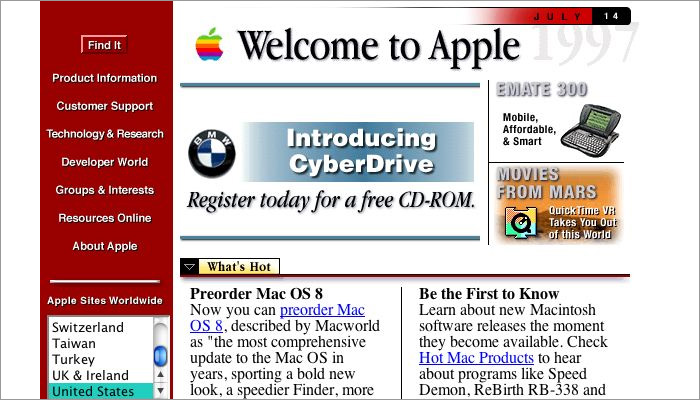
\includegraphics[scale=0.5]{apple.jpg}
	\label{fig:apple}
	\source {\citeonline{appleImg}}
\end{figure}
 

\section{Padrões HTML5}

O \textit{Hyper Text Marking Language} (HTML) é uma linguagem de programação padronizada utilizada para a construção de websites. Desde o ínicio da utilização massiva da internet, a padronização de conteúdo a ser mostrado dentro do HTML foi uma preocupação por parte dos desenvolvedores. Com as ferramentas de pesquisa, essa demanda por padronização se mostrou ainda mais necessária.

Como o padrão foi desenhado em uma época diferente, os propósitos de uma página WEB já não eram mais os mesmos, portanto foi visto a necessidade de mudar as marcações cobertas pela linguagem. Utilizando-se de conceitos previamente desenvolvidos, como \textit{tableless} \cite{tableless} e \textit{navigation}, permitindo ao programador reproduzir explicitamente as marcações de seções e navegações, respectivamente. 

Mecanismos de busca visam procurar dentro dos websites por informações específicas. Preço de produtos, notícias, informações de redes sociais. A gama de funcionalidades e tipo de informações disponíveis em um website aumentou, e a padronização quanto a localidade destas informações se mostrou necessária. 

Como as aplicações já fazem o uso desta padronização visando o agrupamento destas informações, uma aplicação que vise facilitar o uso da Internet por pessoas com inabilidades específicas pode se utilizar destes padrões. 

Duas padronizações particularmente se mostram interessantes. A navegação do usuário, geralmente realizada por ancoras (\textit{links}) dentro do website agora se mostra presente sempre dentro da marcação \textit{nav}. Assim, ao mostrar as opções de navegação e redirecionamento dentro da página, a aplicação pode procurar imediatamente por conteúdos existentes na marcação \textit{nav}, e mostra-las ao usuário, seja em uma forma visual diferente (aumentando as letras, para usuários com dificuldades visuais), ou até mesmo formando alguma maneira de reproduzir em alguma mídia o seu conteúdo, e posteriormente redirecionar o usuário através de comandos simples, diferentes de comandos padrões de usuários (um clique, por exemplo). O Algoritimo \ref{alg:nav-antigo} demonstra como se construia um menu, geralmente feito em um elemento de marcação \textit{ul} (Acrônimo para \textit{Unordered List}). 

\begin{algorithm}[htbp]
	\caption{Exemplo de menu em um modelo HTML anterior ao HTML5}
	\label{alg:nav-antigo}
	\begin{algorithmic}
		\State \textless ul class="menu"\textgreater
			\State \textless li class="menuItem"\textgreater Item 1\textless/li\textgreater
			\State \textless li class="menuItem"\textgreater Item 2\textless/li\textgreater
			\State \textless li class="menuItem"\textgreater Item 3\textless/li\textgreater
			\State \textless li class="menuItem"\textgreater Item 4\textless/li\textgreater
		\State	\textless/ul\textgreater
	\end{algorithmic}
\end{algorithm}

Note que pelo conceito previamente definido, de manter cada marcação HTML exclusivamente trabalhando com questôes para qual a marcação foi construida, utilizar uma lista não é a melhor forma de se manter um menu de navegação em uma página WEB. Também é importante perceber de que a classe CSS definida pode variar, de design para design. Portanto, um website pode definir sua \textit{ul} de navegação com uma classe e outro website com uma classe de nome totalmente distinto. Isto prejudica a procura por padrões por parte das aplicações. O Algoritmo \ref{alg:nav-novo} mostra como a marcação \textit{nav} permite uma padronização mais segura da navegação.

\begin{algorithm}[htbp]
	\caption{Exemplo de menu em HTML5}
	\label{alg:nav-novo}
	\begin{algorithmic}
		\State \textless nav\textgreater
			\State \textless div class="menuItem"\textgreater Item 1\textless/div\textgreater
			\State \textless div class="menuItem"\textgreater Item 2\textless/div\textgreater
			\State \textless div class="menuItem"\textgreater Item 3\textless/div\textgreater
			\State \textless div class="menuItem"\textgreater Item 4\textless/div\textgreater
		\State	\textless/nav\textgreater
	\end{algorithmic}
\end{algorithm}

Também pode-se perceber que não é mais necessário manter os itens do menu como subitens de uma lista. Isto implica uma redução de código CSS, já que cada item presente em uma lista tem um estilo automático gerado, com implicações em posicionamento da tela, identação, espaçamento de linhas, etc. A partir do momento em que cada item dentro da marcação de navegação é apenas uma \textit{div}, esta estilização automática não existe por parte do browser. 

A outra diz respeito à forma com que o conteúdo principal da página é mostrado. Como dito anteriormente, o conceito de \textit{tabless} surgiu antes mesmo do HTML5. Esta prática iniciou-se pois uma diagramação simples das páginas se utilizavam basicamente de tabelas. Porém, o objetivo inicial de uma tabela não condiz com um desenho de uma página por inteiro. Assim, dentro do guia de desenvolvimento padrão de uma página WEB, era inaceitável a utilização de tabelas para a diagramação do \textit{layout} de uma página, sendo indicável a utilização de divisões, ou \textless div\textgreater dentro do \textit{layout}. 

Mas este conceito ainda era insuficiente, mesmo para necessidades básicas de informações no HTML. O próprio exemplo do menu de opções de navegação já demonstra isto. Outro exemplo da ineficiência de utilizar-se apenas divisões é a de páginas com conteúdo escrito denso, ou mesmo páginas com diferentes tipos de conteúdo. 

Páginas de jornais, portais de noticias são exemplos de utulização massiva da marcação \textit{article}. A ideia é manter o conteúdo principal escrito desta página dentro desta marcação.

Outro exemplo refere-se a páginas que possuem várias seções de conteudo diferentes. Muitas páginas procuram dar a experiência do usuário de uma forma corrida e extensa, em uma mesma página, porém, com muitas funcionalidades e conteúdos diferentes. Dai a utilizaçao da marcação \textit{section}, que separa por seções as partes de uma página web.

Com estas divisões bem feitas, facilita-se o trabalho de mecanismos de buscas de conteúdo dentro da página WEB. Os padrões e as indicações feitas pela \citeonline{w3c} vão muito além destas aqui citadas. Porém, pouco acrescentam nas questões específicas de detecção de conteúdo para eventuais mudanças para usuários com inabilidades.

\chapter{Acessibilidade para Usuários com Deficiência Visual} \label{appCegos}

Com os estudos realidados na área de acessibilidade para Deficientes Visuais, o grupo de pesquisa desenvolveu um protótipo simples para demonstrar alguns pontos os quais podem ser úteis para a melhoria da experiência na Internet por parte destes usuários. Algumas tecnologias já existentes no mercado (com conceitos até fora do meio digital) puderam ser aplicados para um exemplo pequeno desta aplicação. Descorreremos através desta unidade, os passos de desenvolvimento desta aplicação protótipo.

\section{Uso do \textit{text-to-speech}}

O conceito de reproduzir textos em áudio não restringe-se ao meio digital. Já há alguns anos, pessoas com deficiência visual tem acesso a ferramentas do dia-a-dia que reproduzem em forma de áudio seu conteúdo, como relógios, agendas eletrônicas, etc. Existem até aplicações \textit{desktop} que realizam este tipo de trabalho para dentro do ambiente do Sistema Operacional. Um exemplo disto é o \citeonline{virtualVision} que funciona dentro do Sistema Operacional trazendo o áudio para o usuário das palavras escritas na tela. 

Existem disponíveis na Internet, ferramentas WEB que reproduzem áudios sobre o conteúdo encontrado no navegador. Estas aplicações (assim como as que funcionam no \textit{desktop}) são chamadas de \textit{text-to-speech}, que como o próprio nome já diz, simplesmente geram áudios do texto definido.

Porém, ainda é necessário analisar qual conteúdo deve ser reproduzido. As ferramentas disponíveis na WEB possuem apenas o formato de biblioteca (ou APIs). Portanto, cabe ao aplicativo que consome estas APIs que reproduzem textos em forma de áudio, qual conteúdo reproduzir.

\subsection{Ferramentas utilizadas}

Tentando desenvolver uma aplicação exatamente para suprir esta demanda, o grupo fez o uso de uma API escrita em \textit{JavaScript} que realiza chamadas simples à biblioteca de sons do Google disponível em seu módulo tradutor \cite{googleTranslate}.

Esta API (\citeonline{responsiveVoice}) se encarrega de fazer as requisições diretamente aos servidores do Google, deixando a iteração com a aplicação em si transparente e de fácil compreensão. O Algorítmo  \ref{alg:algoritmo-exemplo1} apresenta um trecho simples de código que inicia já a aplicação, reproduzindo o conteúdo HTML descrito em um simples elemento HTML. O protótipo final utiliza-se de uma chamada à API idêntica à esta, com diferenciações apenas no momento, e nos elementos em que a chamada é feita.

\begin{algorithm}[htbp]
	\caption{Exempo de chamada simples feita à API ResponsiveVoiceJS}
	\label{alg:algoritmo-exemplo1}
	\begin{algorithmic}
		\Function{ReproduzirTexto}{elemento}
		\State responsiveVoice.speak(elemento.innerHTML);
		\EndFunction
	\end{algorithmic}
\end{algorithm}

Como já citado, a API se encarrega apenas de encapsular chamadas feitas à API do Google Tradutor, e retornar sua resposta. Portanto, a cada conversão \textit{text-to-speech} feita pela API, há uma chamada \citeonline{ajax} feita ao servidor Google. A resposta é automaticamente interpretada pelo navegador como reprodução do arquivo de som recebido, e imediatamente se inicia a reprodução do áudio. 

Para fins técnicos, vale ressaltar que a requisição ao browser é feita por pedaços. Portanto, dependendo do tamanho do texto, mais de uma requisição será feita ao servidor do Google, bem como mais de uma resposta será recebida. O áudio não necessariamente é recebido por inteiro pelo navegador. 

\subsection{Servidor NodeJS}

O \citeonline{nodejs} é uma ferramenta que permite com que os desenvolvedores \textit{JavaScript} utilizem-se da aplicação a fim de criar uma interface do lado Servidor, toda ela escrita na mesma linguagem \textit{JavaScript}. Do lado do desenvolvedor WEB (sobretudo desenvolvedores mais focados em \textit{front-end}), ficou mais fácil se desenvolver aplicações do lado servidor (ou aplicações \textit{back-end}). Também, pela arquitetura assíncrona e diretamente ligada à funções antes tidas apenas do lado cliente, há também a facilidade maior em lidar com requisições HTTP e objetos de transmissão de dados tal qual o \citeonline{json}

O papel principal deste servidor é fornecer a interface inicial ao navegador, e buscar o conteúdo da página WEB desejada. Explicaremos na seção \ref{sec:arquitetura_prototipo} qual é exatamente o papel do servidor, e como analisamos o conteúdo da página web desejada. 

Optamos por utilizar esta ferramenta pela facilidade do grupo em utiliza-la. Porém, não há nela qualquer fator exclusivo que permita a execução do projeto apenas com o uso desta. Alguns fatores como a facilidade de se trabalhar com o objeto JSON deixam o desenvolvimento mais natural. Mas caso a equipe de desenvolvimento opte por utilizar outro tipo de servidor WEB, não há nenhum impedimento. 

\section{Arquitetura do protótipo} \label{sec:arquitetura_prototipo}

Detalharemos aqui a arquitetura geral do protótipo. Vale salientar que esta arquitetura não é de fato a melhor para a resolução do problema. Conceitos de comunicação entre cliente/servidor WEB devem ser levados em conta e melhor tradados durante a aplicação. A aplicação não se encontra \textit{RESTfull} \cite{rest}, que seria a melhor abordagem para o desenvolvimento. Porém, como o objetivo do protótipo era apenas provar conceitos relativos à padronização WEB e a reprodução por meio de áudio de conteúdos escritos, acreditamos que a arquitetura para se utilizar estas ferramentas não fosse importante, como desenvolvimento de prova de conceito. Mas fica claro que em um futuro desenvolvimento de um produto mais robusto, uma arquitetura WEB melhor deve ser adotada.

A Figura \ref{fig:figura-sistema} representa um pedido básico de reprodução de texto. Vale salientar que o inicio do processo se dá no navegador. É nele em que o usuário insere o endereço da página a ser adaptada. Assim, ao confirmar o endereço, a aplicação informa ao servidor (escrito em NodeJS) que esta página é a escolhida. Portanto, o servidor se encarrega de buscar esta página na Internet, simulando uma requisição simples de um navegador. A resposta naturalmente é a própria página, codificada em HTML. Daí, o trabalho do servidor é encontrar as informações necessárias, baseadas numa escolha de padrões dentro da página, como explicaremos na seção \ref{sec:selecao-conteudo}. 

Ao selecionar este conteúdo, o servidor envia de volta para o browser. Recebido, aparece na tela, adicionado como texto simples em uma divisória da página construida, sem qualquer estilo ou \textit{script}. Daí, permite-se ao usuário requisitar a execução do audio do texto. Ao requisitar esta funcionalidade, o navegador faz nova requisição AJAX, mas agora para o servidor do Google Tradutor, enviando o texto a ser reproduzido e a linguagem. O mesmo devolve ao navegador o conteúdo requisitado, e automaticamente o áudio começa a ser executado.

\begin{figure}[htbp]
	\centering
	\caption{Arquitetura geral do sistema}
	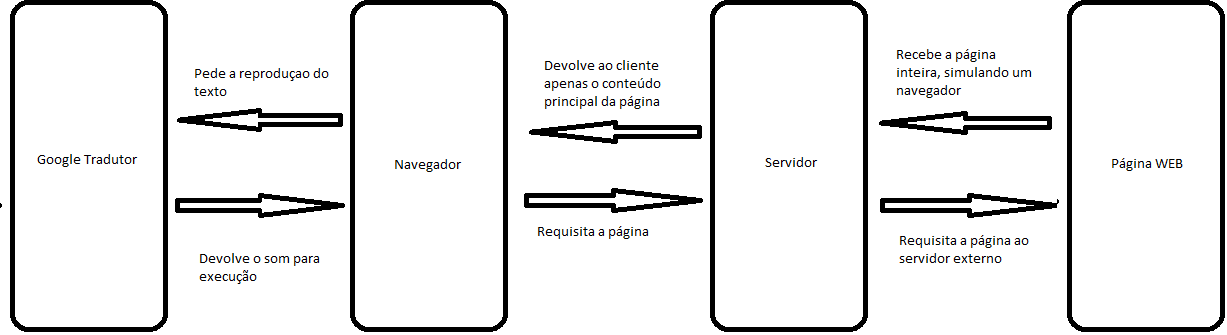
\includegraphics[scale=0.5]{arquitetura_sistema.png}
	\label{fig:figura-sistema}

\end{figure}


\subsection{Seleçao do Conteúdo} \label{sec:selecao-conteudo}

Vale aqui uma breve explicação sobre a escolha do conteúdo feita pela aplicação. Como explicado anteriormente, a padronização por parte da marcação HTML é de extrema importância para que aplicações que buscam interpretar e utilizar parte da página WEB. A aplicação protótipo por nós desenvolvida visa trazer o conteúdo principal da página para ser reproduzido ao usuário, que não possui a capacidade visual de analisar o conteúdo.

Uma página comum de notícia ou blog deve manter seu conteúdo principal dentro das marcações \textit{section} seguidas por uma marcação \textit{article} como mostrada no Algoritmo \ref{alg:algoritmo-exemplo2}. 

\begin{algorithm}[htbp]
	\caption{Exempo de hierarquia ideal de uma página HTML5}
	\label{alg:algoritmo-exemplo2}
	\begin{algorithmic}
	\State \textless section class="menuWrapper"\textgreater
		\State \textless nav class="menuItem"\textgreater
		\State ... 
		\State ...
	\State	\textless/nav\textgreater
	\State \textless/section\textgreater
	\State ...
	\State ...
	
	\State \textless section class="articleWrapper"\textgreater
	\State 		\textless article class="articleContent"\textgreater
	\State 			\textless p\textgreater
	\State 				Conteudo principal do artigo...
		\State		\textless/p\textgreater
	\State		\textless/article\textgreater
	\State \textless/section\textgreater

	\end{algorithmic}
\end{algorithm}

Podemos ver que a marcação \textit{section} separa as principais seções da página. E a marcação \textit{article} contém o conteúdo principal. Assim, o servidor da aplicação desenvolvida busca retornar ao navegador apenas o conteúdo dentro desta marcação \textit{article}, com ou sem as marcações adicionais de parágrafo (conhecida como a marcação \textit{p}).
 
O algoritmo \ref{alg:algoritmo-exemplo3} mostra simplificadamente como ficaria uma seleção por \textit{JavaScript} deste conteúdo, retornando-o para um uso qualquer de um consumidor desta função.

\begin{algorithm}[htbp]
	\caption{Exempo de seleção simples de conteúdo principal de um artigo WEB}
	\label{alg:algoritmo-exemplo3}
	\begin{algorithmic}
		\Function{SelecionarCOnteudo}{elemento}
		\State var contentArray = document.getElementsByTagName("article").
		\State var textContent = "";
		\For{var i = 0; i < contentArray.length; i++}
		\State	textContent += contentArray[i].innerHTML;
		\EndFor
		
		\Return return textContent
		\EndFunction
	\end{algorithmic}
\end{algorithm}

Este exemplo retorna todo o conteúdo dentro da marcação \textit{article}, o que traz também a marcação \textit{p} em formato texto, de forma indesejada. O protótipo desenvolvido utiliza \citeonline{JQuery} que facilita a retirada das marcações, e consegue selecionar apenas o texto. Outro item utilizado pela aplicação foi a seleção da marcação \textit{h}, que guarda o título do texto, e é de vital importância para a compreensão do texto em áudio. 

\subsection{Dificuldades na seleção do conteúdo}

Como o conteúdo principal de uma página de um artigo jornalístico por exemplo se refere apenas o conteúdo da reportagem e suas imagens. Para um usuário com deficiências visuais, a imagem em sí não interessa, tampouco os demais itens, como propagandas, iterações de redes sociais, etc. A seleção da marcação article já seria o suficiente em um mundo ideal, porém há um problema de padronização por parte dos portais de notícias do mundo. Muitos ainda não aderiram ao formato HTML5 de marcações, e também incluem conteúdos que não interessam ao usuário, como número de comentários em redes sociais, anchoras para compartilhamento em aplicativos de mensagem, etc. A solução temporária foi analisar padrões específicos de cada portal de noticia e realizar uma pesquisa pelas marcações existentes nesses padrões analisados. 

\begin{algorithm}[htbp]
\caption{Seleção dos elementos HTML de acordo com o dominio da página}
	\label{alg:algoritmo-exemplo4}
	\begin{algorithmic}
		\State var htmlPatterns = \{
		\State	"folha.uol.com.br": "article\textgreater .content\textgreater p",
		\State	"uol.com.br": "article\textgreater header\textgreater h1, article\textgreater\#texto\textgreater p, article\textgreater\#texto\textgreater h3",
		\State	"estadao.com.br":"h2.titulo-principal, div.content\textgreater p",
		\State	".":"article"
		\State \}; 
	
		\Function{SelecionarConteudo}{} \{
		\State var contentArray = \$(htmlPatterns[window.location.href]).
		\State var textContent = contentArray.text();
		
		\Return return textContent;
		\EndFunction
		\}
	\end{algorithmic}
\end{algorithm}


\subsection{Melhorias na aplicação}

A Figura \ref{fig:figura-interface} demosntra a interface geral da aplicação. Página de simples diagramação, o objetivo principal é manter as funcionalidades de fácil acesso para um eventual auxílio externo, ou pelo próprio comando do usuário. A aplicação permite que o usuário apenas use o teclado para disparar a ação de leitura do áudio, sem a necessidade da utilização do mouse.

\begin{figure}[htbp]
	\centering
	\caption{Layout da página protótipo}
	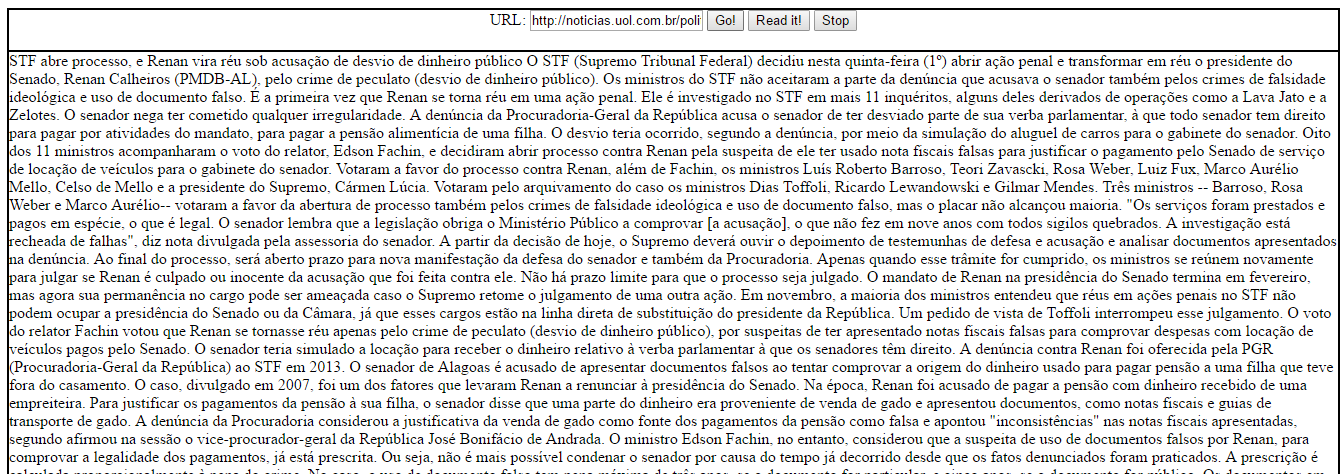
\includegraphics[scale=0.4]{figura-interface.png}
	\label{fig:figura-interface}
	
\end{figure}

Mas há ainda muito espaço para melhorias. Como o protótipo foi criado apenas com o intuito de prova de conceito, há ainda muitos detalhes de acessibilidade que devem ser abordados. Traremos aqui alguns pontos que no desenvolvimento final do produto, podem apresentar melhorias substanciais para os usuários do sistema.

Fica claro na representação da aplicação que a utilização da aplicação é extremamente limitada ao usuário com deficiências auditivas. Fica necessário a presença de uma aplicação independente do navegador. O trabalho inicial que o usuário teria para apenas abrir o navegador seria gigantesco. Portanto, uma aplicação completa deve possuir um trabalho específico para que não haja a necessidade de um navegador desta maneira (pelo menos na maneira geral apresentada). 

Duas alternativas podem existir para a resolução deste problema. A primeira é adaptar uma aplicação de navegação WEB para este propósito. A outra é na verdade nem utilizar o navegador. A reprodução do áudio pode ficar a cargo do Sistema Operacional e de suas ferramentas, desde que haja um cliente WEB suficientemente inteligente para separar o áudio recebido na requisição ao servidor do Google Tradutor da mensagem, e executar o comando no Sistema Operacional.

No protótipo, existem apenas estudos de padrões para três portais WEB. Seria necessário em um primeiro momento, dar suporte para mais páginas WEB, de uso tradicional pela sociedade. A \textit{priori}, este comportamento deveria poder ser generalizado pela padronização WEB ideal. Porém, em um meio tão diversificado de desenvolvimento, se mostra praticamente impossível uma pesquisa por elementos genérica para todo e qualquer página WEB. 

Possívelmente, uma análise sobre inserção de novos padrões pelo próprio usuário, poderia trazer uma melhor abrangência do sistema sobre as páginas WEB dispostas na Internet, sob um modelo semelhante ao usado por \citeonline{socialAll}. A inserção destes padrões deve ser feita de forma fácil ao usuário comum, de forma que este não possui necessariamente conhecimentos técnicos sobre programação \textit{front-end}.

Também fica claro que este modelo não permite nenhuma nevegação por parte do usuário com inabilidade visual. Este problema requer um estudo mais aprofundado sobre ferramentas já existentes que facilitam a utilização do computador pelo usuário deficiente visual. Mas um caminho a ser seguido é o de comandos pelo teclado, algo brevemente implementado no protótipo.

Os controles de inicio e término da ação de leitura são indicios de que o usuário também pode usar o teclado para navegação. Daí a importância da padronização da marcação \textit{nav}, já que seria nela que os elementos de menu estariam dispostos. Assim, seria possivel que uma aplicação recupere os elementos ali presentes juntamente com as anchoras necessárias, e portanto ao comando do teclado, o usuário poderia escolher para onde quer ser redirecionado. 

\chapter{Acessibilidade para Usuários com Deficiência Auditiva}

O protótipo apresentado para o projeto de página WEB acessível para usuários com deficiência auditiva é apenas uma aplição estática que demonstra pontos que podem ser abordados dinâmicamente por uma aplicação completa e robusta. Utilizando os conceitos apresentados por \citeonline{deafPeople} e pela \citeonline{w3cWai}, apresentamos formas de ajuda aos usuários que podem eventualmente se aproveitar em uma página WEB que aplique estes conceitos, ou até de aplicações que apliquem estes conceitos, utilizando apenas o conteúdo da página WEB, como realizado no protótipo apresentado no capitulo \ref{appCegos}.

\section{Troca de palavras por sinônimos}

\citeonline{deafPeople} citam a dificuldade que pessoas com inabilidades auditivas tem de compreensão de texto. Cita que a leitura está diretamente conectada a escuta, e que os significados muitas vezes se entrelaçam com a entonação ou com a fonética. Portanto, usuários com problemas auditivos podem ter mais problemas na interpretação de texto devido a problemas com o significado de algumas palavras.

Pensando nisto, um dicionário de sinônimos pode ser útil para o usuário. Porém, um dicionário de busca pode ser inconveniente ao uso da aplicação. Como o usuário já volta suas atenções à página, uma mostragem de sinônimos que siga o fluxo de leitura do usuário é mais conveniente à usabilidade. 

A Figura \ref{fig:prototipoSinonimo} demonstra o  protótipo de sinônimo trazido ao usuário ao momento de consulta. Utilizou-se uma anchora e um evento para que no momento em que o usuário pare o \textit{mouse} sobre o objeto, uma aba apareça, com o sinônimo da palavra desejada. Segundo \citeonline{deafPeople}, esta ajuda facilita a execução de tarefas em uma página WEB por parte dos usuários com deficiência auditiva, já que pode fornecer palavras conhecidas ao usuário, facilitando sua compreensão. Vale também a observação que esta alternativa, se automátizada, pode trazer também vantagens para usuários que não possuem a primeira língua igual à lingua da página WEB, ou até usuários com deficiências no aprendizado.

\begin{figure}[htbp]
	\centering
	\caption{Demonstração da aplicação com sinônimos}
	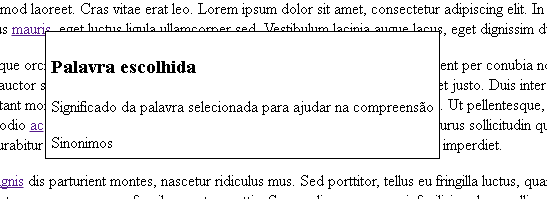
\includegraphics{prototipoCego.png}
	\label{fig:prototipoSinonimo}

\end{figure}

De forma semelhante, podemos inserir também à ajuda de sinônimos, o mesmo conteúdo escrito, mas em linguagem de sinais. Com todas as ressalvas sobre a dificuldade de padronização da linguagem (como definido na seção \ref{libras}), uma apresentação da palavra nesta linguagem reduz substancialmente o tempo de execução de tarefa, e melhora a análise sobre a página pelo usuário \cite{deafPeople}. A Figura \ref{fig:prototipoLibra} demonstra como ficaria a adição da figura à ajuda de sinônimos no layout da página.

\begin{figure}[htbp]
	\centering
	\caption{Demonstração da aplicação com sinônimos e a palavra equivalente em Libras}
	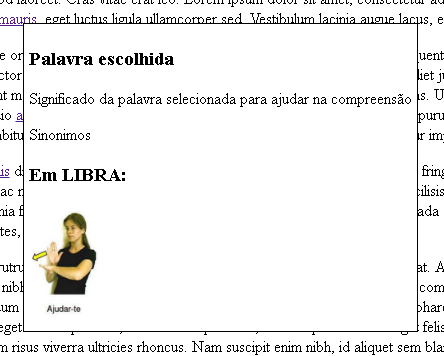
\includegraphics{prototipoLibra.png}
	\label{fig:prototipoLibra}
\end{figure}

\section{Redução e Resumo do texto}

\citeonline{deafPeople} também citam que o usuário pode se perder em textos muito extensos. Este fator na verdade aplica-se para todo e qualquer tipo de usuário, como exemplificado pelos padrões de acessibilidade da \citeonline{w3c}. Porém, este problema pode ser agravado quando o usuário possui alguma inabilidade, seja ela qual for, já que o estresse de se utilizar uma aplicação que não lhe é confortável prejudica ainda mais seu desempenho no sistema. 

Por meio de uma análise semântica, é possível se analisar trechos do texto que podem ser descartados, reduzindo seu tamanho. Mas não é apenas este problema que uma análise profunda do texto pode fazer. Quando se trata de linguagem escrita independente da linguagem falada, há uma dificuldade de compreensão quando se trata de algumas classes de palavras ou sentenças, como conjunções, advérbios, etc. A análise textual pode modificar o texto de forma com que estas palavras possam ser melhor recebidas pelo usuário, inseridos em algum contexto específico.

Nosso protótipo demonstra como a aplicação pode se comportar com um algorimtmo de Processamento de Linguagem natural (como descrito na seção \ref{nlp}). Uma ação do usuário (neste caso, um clique no botão) faz com que o conteúdo da página seja analisado e transformado de acordo com o padrão estabelecido.

\chapter{Conclusão}

Há um espaço gigantesco a ser preenchido pelos desenvolvedores quando o assunto é acessibilidade para usuários com inabilidades especificas. Não há uma preocupação por desenvolvedores para com este público alvo, que apesar de em menor número, devem ser incluídos neste meio digital. Existem padrões especificados pela \citeonline{w3cWai} que dizem por exemplo que autores de \textit{podcasts} deveriam inserir a transcrição do texto juntamente com o áudio fornecido, para assim, ser considerado acessível. Com as ferramentas disponíveis na Internet de transcriçao de áudio e de forma gratuita, estes problemas mais simples poderiam ser resolvidos pelos próprios desenvolvedores ou definidores de conteúdo das páginas WEB deste tipo.

Para um desenvolvimento automático de ferramentas que possam facilitar esta inclusão, há ainda um problema que ultrapassa as intenções deste feito. Uma padronização geral de desenvolvimento WEB seria o principal motor para um desenvolvimento robusto e abrangente de ferramentas deste tipo. Porém, como no desenvolvimento de qualquer sistema, é natural a dificuldade de padronização, sobretudo padronização que atinja uma gama de desenvolvedores em múltiplas organizações, países, etc. 

Mas ainda sim, vimos que é possível com que haja esta preocupação por parte dos principais portais de internet quando o assunto é acessibilidade. É possível que páginas se preocupem com uma automatização de seus próprios conteúdos para dar suporte à este tipo de necessidade, já que a busca por padrões dentro de uma só organização é muito mais simples e prática. Mas ainda de uma forma geral, há problemas de cumprimento de regras estabelecidas pela \citeonline{w3c} para HTML5 básico. 


% ----------------------------------------------------------
% ELEMENTOS PÓS-TEXTUAIS
% ----------------------------------------------------------
\postextual
% ----------------------------------------------------------

% ----------------------------------------------------------
% Referências bibliográficas
% ----------------------------------------------------------
\bibliography{referencias}


%---------------------------------------------------------------------
% INDICE REMISSIVO
%---------------------------------------------------------------------
%%%%%MF\phantompart
%%%%%MF\printindex
%---------------------------------------------------------------------

\end{document}
